\documentclass[11pt]{article}
\usepackage[T1]{fontenc}
\usepackage{amsmath,amssymb,amsthm,booktabs,geometry}
\usepackage{pgfplots}
\pgfplotsset{compat=1.18}
\usepackage[colorlinks=true,linkcolor=blue,urlcolor=blue,citecolor=blue]{hyperref}
\geometry{margin=1in}
\newtheorem{theorem}{Theorem}
\newtheorem{lemma}[theorem]{Lemma}
\newtheorem{corollary}[theorem]{Corollary}
\newcommand{\pos}[1]{\left(#1\right)_+}
\newcommand{\dd}{\,\mathrm d}
\newcommand{\Core}{\mathcal C}
\newcommand{\G}{\mathcal G}
\title{A cutoff law for a class-subtracted prime-power core}
\author{increasezerozeta project}
\date{October 2026 --- research draft}
\begin{document}
\maketitle
\begin{abstract}
We compute the complete cutoff distribution of an explicitly defined
class-subtracted prime-power model motivated by a fourth-moment
calculation for the Riemann zeta function. For a modulus cutoff
$\exp(\delta\ell)$, the normalized core equals $c(\delta)+O(\ell^{-1})$,
uniformly for $0\leq\delta\leq1$. The function $c$ is piecewise polynomial
of degree five, with transitions at $1/3$, $1/2$ and $2/3$.
The same formula holds for a cutoff on both reduced dilations.
The leading core is $-1/48$; a cube-root cutoff captures only $59/1215$
of it. We derive the formula from a clipped-cube volume and provide
independent exact rational checks against the original twelve overlaps.
This is a theorem about the specified arithmetic model. Its identification
with an actual zeta moment remains a separate analytic problem.
\end{abstract}

\section{Statement and range implications}
Put $\ell=\log(T/(2\pi))$ and $\ell_1=\ell+2\log2-1$.
The core $\Core_\ell$, defined precisely in Section~\ref{sec:model},
has total leading term $-1/48$. For $B=\exp(\delta\ell)$, let
$\Core_\ell[B]$ restrict its modulus atoms to $b_1,b_2\leq B$.
For $g=\gcd(b_1,b_2)$, write $r=b_1/g$, $q=b_2/g$; let
$\Core_\ell^{\rm red}[B]$ instead restrict $\max(r,q)\leq B$.

\begin{theorem}\label{thm:main}
Uniformly for $0\leq\delta\leq1$,
\[
 \Core_\ell[\exp(\delta\ell)]
 =c(\delta)+O(\ell^{-1}),\qquad
 \Core_\ell^{\rm red}[\exp(\delta\ell)]
 =c(\delta)+O(\ell^{-1}),
\]
where
\[
c(\delta)=
\begin{cases}
-\dfrac{59\delta^5}{240},&0\leq\delta\leq\frac13,\\[4pt]
-\dfrac{59\delta^5}{240}+\dfrac{(3\delta-1)^5}{60},
 &\frac13\leq\delta\leq\frac12,\\[4pt]
-\dfrac1{48}+\dfrac{2(1-\delta)^4}{3}
 -\dfrac{14(1-\delta)^5}{15}
 +\dfrac{(11\delta-4)(2-3\delta)^4}{80},
 &\frac12\leq\delta\leq\frac23,\\[4pt]
-\dfrac1{48}+\dfrac{2(1-\delta)^4}{3}
 -\dfrac{14(1-\delta)^5}{15},
 &\frac23\leq\delta\leq1.
\end{cases}
\]
\end{theorem}

The fraction of the leading core captured is $F(\delta)=-48c(\delta)$.
It increases continuously and strictly from zero to one. In particular,
\[
 F(1/3)=\frac{59}{1215},\quad F(1/2)=\frac{11}{32},\quad
 F(2/3)=\frac{959}{1215},\quad F(3/4)=\frac{147}{160}.
\]
For $\delta\geq2/3$ its remaining fraction has the exact form
\begin{equation}\label{eq:tail}
 1-F(\delta)=32(1-\delta)^4-\frac{224}{5}(1-\delta)^5.
\end{equation}

\begin{corollary}
If $\log B=o(\ell)$, then $\Core_\ell^{\rm red}[B]=o(1)$, and
the complementary region retains $-1/48+o(1)$.
\end{corollary}
\begin{proof}
Take $\delta=\log B/\ell$ in the uniform theorem.
\end{proof}

Recovering the leading model term by covering the restricted dilation
region therefore requires a positive-power range. Exact rational
bisection gives the following brackets for the inverse of $F$:
\begin{center}
\begin{tabular}{cc}
\toprule
Leading fraction & Cutoff exponent interval\\
\midrule
$1/2$ & $(0.551320,\,0.551321]$\\
$9/10$ & $(0.734423,\,0.734424]$\\
$99/100$ & $(0.859563,\,0.859564]$\\
\bottomrule
\end{tabular}
\end{center}
These are exponents relative to $\exp(\ell)=T/(2\pi)$, not to a
progression-window length. A different global analytic argument could
avoid region-by-region transport; the theorem does not exclude that.

\begin{center}
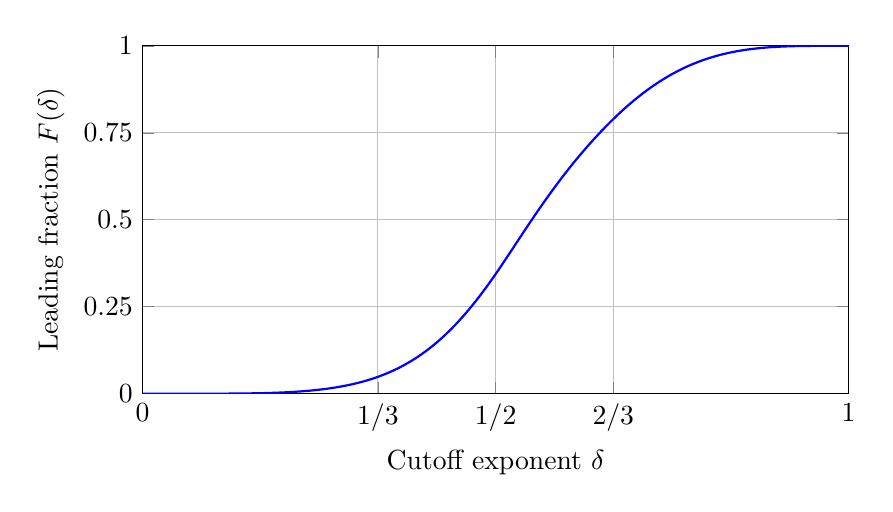
\begin{tikzpicture}
\begin{axis}[width=.87\textwidth,height=6cm,
 xlabel={Cutoff exponent $\delta$},ylabel={Leading fraction $F(\delta)$},
 xmin=0,xmax=1,ymin=0,ymax=1,grid=major,
 xtick={0,.333333333,.5,.666666667,1},
 xticklabels={$0$,$1/3$,$1/2$,$2/3$,$1$},
 ytick={0,.25,.5,.75,1},samples=101]
\addplot[blue,thick,domain=0:1/3] {59*x^5/5};
\addplot[blue,thick,domain=1/3:1/2] {59*x^5/5-4*(3*x-1)^5/5};
\addplot[blue,thick,domain=1/2:2/3]
 {1-32*(1-x)^4+224*(1-x)^5/5-3*(11*x-4)*(2-3*x)^4/5};
\addplot[blue,thick,domain=2/3:1]
 {1-32*(1-x)^4+224*(1-x)^5/5};
\end{axis}
\end{tikzpicture}
\end{center}
The plot evaluates the explicit formulas; it is not numerical evidence
for the asymptotic theorem.

\section{The specified model}\label{sec:model}
We retain the coefficient and ordered overlap conventions of the
pinned reference implementation~\cite{reference}. For a prime $p$ put
$e_i=v_p(b_i)$, $e=\min(e_1,e_2)$ and $\alpha=(p-1)^{-1}$.
The local coefficient measure is supported at $p^e,p^{e+1}$, with
respective coefficients
\[
 (1-\alpha^2,\alpha^2)\quad(e_1=e_2),\qquad
 (1+\alpha,-\alpha)\quad(e_1\ne e_2).
\]
Let $S$ be the primes dividing $2b_1b_2$. Denote by $\eta$ the finite
tensor of these vectors over $S$, and by $R$ the tensor of the ordinary
positive vectors over odd primes outside $S$. Multiplicative
convolution defines the class-subtracted measure
\[
 \gamma^{b_1,b_2}=\eta*R-\eta.
\]
The subtraction is part of the model definition. For prime-power
$b_i$ there are at most two special odd primes, and
$\sum_d|\gamma_d^{b_1,b_2}|\leq24$.

For a real argument $y$, define
\[
 A(y)=
 \begin{cases}
 0,&y\in2\pi\mathbb Z,\\
 (\pi-(y\bmod2\pi))/2,&y\notin2\pi\mathbb Z,
 \end{cases}
 \qquad G_0(x)=2\bigl(A(2x)-A(x)\bigr).
\]
Thus $G_0(x)=-x$ for $0<x<\pi$ and $|G_0(x)|\leq\pi$.
The absolutely convergent transform is
\[
 \G_{b_1,b_2}(\theta)=\sum_d\gamma_d^{b_1,b_2}G_0(d\theta).
\]
With $\Lambda$ the von Mangoldt function, put
\[
 \mu_\ell=\frac1\ell\sum_{b\leq e^\ell}\frac{\Lambda(b)}b
           \delta_{\log b/\ell},\qquad
 \theta=2\pi e^{-(\nu-1)\ell},\quad
 D_\nu=[\nu-1,\nu/2]^2,\quad 1\leq\nu\leq2.
\]
Let $O(v_1,\ldots,v_4)=(1-\max v_i+\min v_i)_+$.
The original twelve-overlap function $H(\beta_1,\beta_2,\nu)$ sums
\[
 O(0,-a,c-d,-d)+O(0,b-c-d,-c-d,-d)
                    +O(0,-b-c+d,-c+d,d)
\]
over $(a,c)=(\beta_1,\nu-\beta_1),(\nu-\beta_1,\beta_1)$ and
$(b,d)=(\beta_2,\nu-\beta_2),(\nu-\beta_2,\beta_2)$.
In every case $a+c=b+d=\nu$.
The core is
\begin{equation}\label{eq:core}
 \Core_\ell=
 2\left(\frac{\ell}{\ell_1}\right)^4
 \int_1^2\int_{D_\nu}
 \frac{\G_{b_1,b_2}(\theta)}{\theta\ell}
 H(\beta_1,\beta_2,\nu)\,
 \dd\mu_\ell(\beta_1)\dd\mu_\ell(\beta_2)\dd\nu.
\end{equation}
At the atoms $b_i=e^{\ell\beta_i}$. Cutoffs restrict these atoms;
the continuum formulas below describe their limit.

\section{Arithmetic reduction and uniformity in the cutoff}
We record the arithmetic ingredients from the quantitative core
proof~\cite{core}, including why they remain uniform after a cutoff.
The classical Mertens estimate~\cite{mertens} gives
\begin{equation}\label{eq:mertens}
 \sup_{0\leq x\leq1}|\mu_\ell([0,x])-x|=O(\ell^{-1}).
\end{equation}
For the universal $(1,1)$ class the full coefficients are
\[
 \Gamma_{2m}^{1,1}=C_2\prod_{p\mid m}\frac1{p(p-2)}
\]
on odd squarefree $m$, with $C_2=\prod_{p>2}(1-(p-1)^{-2})$;
the class subtraction is $\delta_2$.
The auxiliary function $a(m)=\prod_{p\mid m}(p-2)^{-1}$ has the
Dirichlet convolution $a=(1/{\rm id})*h$, where
\[
 h(2)=-\tfrac12,\qquad h(p)=\frac2{p(p-2)},\qquad
 h(p^2)=-\frac1{p(p-2)}\quad(p>2).
\]
All other nontrivial prime-power coefficients vanish.
For every $0<\alpha<1/2$, $\sum|h(d)|d^\alpha<\infty$.
The harmonic-number expansion and partial summation consequently give
\[
 \sum_{d\leq M}d\gamma_d^{1,1}
 =\log M+\gamma_{\rm E}-2
   +O_\alpha(M^{-\alpha}(1+\log M)),\qquad
 \sum_{d>M}\gamma_d^{1,1}
 =M^{-1}+O_\alpha(M^{-1-\alpha}(1+\log M)).
\]
Splitting the transform at $d\asymp\theta^{-1}$ proves
$\G_{1,1}(\theta)=-\theta\log(1/\theta)+O(\theta)$.

For distinct ordinary odd primes $p,q$, comparison of the two
special local vectors with the ordinary vectors, including the
subtraction, gives
$\|\gamma^{p,q}-\gamma^{1,1}\|_1\leq12(1/p+1/q)$.
On $D_\nu$ one has $p,q\geq2\pi/\theta$. Hence
$|\G_{p,q}-\G_{1,1}|\leq12\theta$, and uniformly throughout the region,
\begin{equation}\label{eq:ordinary}
 \frac{\G_{p,q}(\theta)}{\theta\ell}
 =-(\nu-1)+O(\ell^{-1}).
\end{equation}
The coprime prime-power estimate
$\sum_{d\leq M}d|\gamma_d|\ll1+\log M$ gives
$|\G(\theta)/(\theta\ell)|\ll\nu-1+\ell^{-1}$ uniformly.
Higher prime powers and the atom at $2$ have $\mu_\ell$ mass
$O(\ell^{-1})$, so coprime exceptions contribute that amount absolutely.
The local weighted bound follows by bounding the special tensor's
weighted absolute mass by $36$ and removing at most two ordinary odd
factors from the universal positive tensor; the bounds are independent
of the positive exponents of the coprime moduli.

Shared-base pairs use $\sum|\gamma_d|\leq24$ instead. Their allowed
$\nu$ range ends at $1+\log\min(b_1,b_2)/\ell$. Integration of
$\theta^{-1}$ bounds their full absolute contribution by
\[
 O\left(\ell^{-4}
 \sum_{p^a,p^b\leq e^\ell}\frac{(\log p)^2}{p^{\max(a,b)}}\right)
 =O(\ell^{-2}).
\]
Indeed the exponent-one sum is $O(\ell^2)$ by Mertens, while
$\sum_{k\geq2}(2k-1)/p^k\ll p^{-2}$ and
$\sum_p(\log p)^2/p^2<\infty$. Every restricted subset satisfies
the same absolute bound.

The function $H$ is bounded and has uniformly bounded piecewise affine
variation in each coordinate. Restricting a coordinate interval at
$\delta$ adds at most one bounded jump. Applying integration by parts
twice to~\eqref{eq:mertens}, including endpoint atoms, therefore gives
an $O(\ell^{-1})$ product-measure error independent of $\delta$.
Removing exceptions with the absolute estimates above, and using
$(\ell/\ell_1)^4=1+O(\ell^{-1})$, reduces the theorem to
\begin{equation}\label{eq:reduction}
 \Core_\ell[e^{\delta\ell}]
 =-2\int_0^\delta u Q_\delta(1+u)\dd u+O(\ell^{-1}).
\end{equation}
Here $Q_\delta$ is the integral of $H$ over
$[\nu-1,\min(\delta,\nu/2)]^2$, interpreted as zero when empty.

\section{A clipped-cube identity for all branches}
The original overlaps give the ordered formula
\[
 H=4(1-\nu+\min(\beta_1,\beta_2))
   +2\sum_{c\in\{\beta_1,\nu-\beta_1\}}
       \sum_{b\in\{\beta_2,\nu-\beta_2\}}
                   (1-\max(\nu+c-b,b))_+.
\]
Set $\nu=1+u$, $\beta_1=u+x$, $\beta_2=u+y$ and
$t=\min(\delta-u,(1-u)/2)$.
On $[0,t]^2$ the four swapped terms become
\[
 (y-x-u)_+,\quad\min(y,1-2u-x-y)_+,\quad0,\quad
 \min(x-y-u,y)_+.
\]
The first and last integrals are $(t-u)_+^3/6$ and
$(t-u)_+^3/12$; also $\int4\min(x,y)=4t^3/3$.
For the remaining term put $s=1-2u$ and introduce a height $z$.
Its integral is the volume of
\[
 0\leq x\leq t,\quad0\leq z\leq y\leq t,\quad x+y+z\leq s.
\]
Exchange of $y,z$ bisects the clipped cube. Inclusion-exclusion on
its three upper faces proves
\begin{equation}\label{eq:q}
 Q_\delta(1+u)=\frac{4t^3}{3}+\frac{(t-u)_+^3}{2}
 +\frac{s_+^3-3(s-t)_+^3+3(s-2t)_+^3-(s-3t)_+^3}{6}.
\end{equation}
For the full side $t=(1-u)/2$, the $(1-3u)_+^3$ terms cancel and
$Q_1(1+u)=((1-u)^3+(1-2u)_+^3)/6$. Its weighted integral is $1/96$.

When $\delta\leq1/2$, the side is $\delta-u$. The four cube arguments
are $1-2u$, $1-\delta-u$, $1-2\delta$ and $1-3\delta+u$.
The first three remain nonnegative over $[0,\delta]$. The fourth
changes sign only for $\delta>1/3$. Direct integration gives
\[
 -2\int_0^\delta u Q_\delta(1+u)\dd u
 =-\frac{59\delta^5}{240}+\frac{(3\delta-1)_+^5}{60}.
\]
The correction follows by replacing the full cubic by its positive
part: the omitted negative integral is $-(3\delta-1)^5/20$.

For $\delta\geq1/2$, put $\eta=1-\delta$ and $a=2\delta-1$.
The side is full on $[0,a]$ and is $\delta-u$ on $[a,\delta]$.
The term $(1-2u)_+^3/6$ has total weighted integral $1/480$.
The two first terms have total weighted integral
\[
 \int_0^a \frac{u(1-u)^3}{6}\dd u
 +\int_a^\delta \frac43u(\delta-u)^3\dd u
 =\frac1{120}-\frac{\eta^4}{3}+\frac{7\eta^5}{15}.
\]
The remaining correction is
\[
 \frac12\int_a^\delta u\bigl((\delta-2u)_+^3
                           -(1-\delta-u)_+^3\bigr)\dd u.
\]
It vanishes for $\delta\geq2/3$. Otherwise put $b=2-3\delta$ and
$u=a+v$. The two upper limits are $b/2,b$, and the difference equals
\[
 -\frac{ab^4}{16}-\frac{3b^5}{160}
 =-\frac{(11\delta-4)b^4}{160}.
\]
Combining and multiplying by $-2$ proves the last two branches in
Theorem~\ref{thm:main}. Different-base prime-power atoms have $g=1$;
the modulus and reduced-dilation cutoffs differ only on shared-base
pairs, whose full absolute contribution is $O(\ell^{-2})$.
This completes the proof of both assertions.

\section{Distribution, verification and scope}
The positive measure $96uH\,\dd\beta_1\dd\beta_2\dd u$ on the full region
has total mass one. Its distribution of $\max(\beta_1,\beta_2)$ is $F$.
Differentiation on the four branches gives respectively
\[
 59\delta^4,\quad59\delta^4-12(3\delta-1)^4,\quad
 (1-\delta)^3(224\delta-96)
       +\frac35(2-3\delta)^3(165\delta-70),\quad
 (1-\delta)^3(224\delta-96).
\]
These are positive in the interiors, and the branch formulas agree
at their endpoints. This proves strict monotonicity and justifies
unique quantiles and rational bisection.

The standard-library reproduction commands are
\begin{verbatim}
python scripts/verify_arithmetic_transport.py
python scripts/verify_dilation_coverage.py
python scripts/verify_project.py
\end{verbatim}
The cutoff checker integrates the original twelve overlaps by exact
rational polygon clipping at 86 configurations. A separate univariate
integrator splits~\eqref{eq:q} at its actual affine roots and checks
61 rational cutoff exponents. It also verifies 1620 pointwise overlap
identities, exact coverage fractions, the displayed quantile brackets
and 1536 reduced-cutoff classifications. Symbolic polynomial arithmetic
checks the four density identities and exact branch joins. No coefficient is obtained by
fitting those samples. The analytic argument is the proof above,
with the coefficient estimates detailed in the companion core note.

The coefficient and overlap convention is credited to the reference
implementation. Mertens' estimate is classical. The cutoff assembly
and clipped-cube derivation are developed in this project; independent
review and priority assessment remain necessary. Derivations and code
were developed with AI assistance. The tests check finite identities
and do not replace mathematical review or limiting arguments.

The cutoff here is on physical moduli and reduced dilations. It differs
from a Ramanujan-denominator cutoff. The result does not prove a
prime-correlation estimate in the positive-power dilation range,
a signed actual-minus-model discrepancy, or the reduction of an
actual zeta moment to~\eqref{eq:core}. Those obligations remain separate.

\begin{thebibliography}{9}
\bibitem{reference}
JoshuaHKU, \emph{zeta-0.7947-reproduction}, revision
\texttt{d85bddfe9d8f12856fba735fc9cb3ca23b48b3a8}.
Coefficient convention in \texttt{mains\_envelope.py} and
\texttt{tail\_bound.py}; twelve-overlap geometry and sawtooth in
\texttt{m1\_suite.py}.
\url{https://github.com/JoshuaHKU/zeta-0.7947-reproduction/tree/d85bddfe9d8f12856fba735fc9cb3ca23b48b3a8}.

\bibitem{core}
increasezerozeta project, \emph{A quantitative limit for the
class-subtracted arithmetic core}, companion proof note.
\url{https://github.com/Aky-lab/increasezerozeta/blob/main/notes/arithmetic_core_limit.md}.

\bibitem{mertens}
MIT 18.785, Fall 2021, \emph{Problem Set 9}, Problem 1.
\url{https://ocw.mit.edu/courses/18-785-number-theory-i-fall-2021/mit18_785f21_pset9.pdf}.

\bibitem{reproduction}
increasezerozeta project, \emph{The full dilation distribution of the
arithmetic core}, proof note and exact verification source.
\url{https://github.com/Aky-lab/increasezerozeta/blob/main/notes/dilation_core_coverage.md}.
\end{thebibliography}
\end{document}
